\section{Experimentelles Vorgehen und Ergebnisse}
\subsection{Abhängigkeit der Aktingeschwindigkeit von der Konzentration des ATP}
Für die während der Versuchsvorbereitung erstellten Messproben wurden mit dem Mikroskop und einer CCD Kamera für verschiedene ATP-Konzentrationen alle
100 ms insgesamt 100 Bilder aufgenommen. Mithilfe des Programms "ImageJ" konnte man die Geschwindigkeit
der Aktinfilamente bestimmen. Dabei wurden die Geschwindigkeit jener Aktinfilamente gemessen, die
sich über die Zeit von 100ms kontinuierlich bewegt haben. Bei höheren Konzentrationen von ATP war die
Geschwindigkeit der Aktinfilamente deutlich höher als bei niedriegen Konzentrationen,
wie durch die Michaelis-Menten Gleichung \ref{equ:michaelis_menten} vorhergesagt.
Jedoch zeigt der letzte Messpunkt bei der ATP Stoffmenge von 2000$\mu \text{Mol}$ eine starke
Abweichung vom geplottetem Graphen \ref{fig:normal_speed}.
\begin{figure}[h]
  \centering
  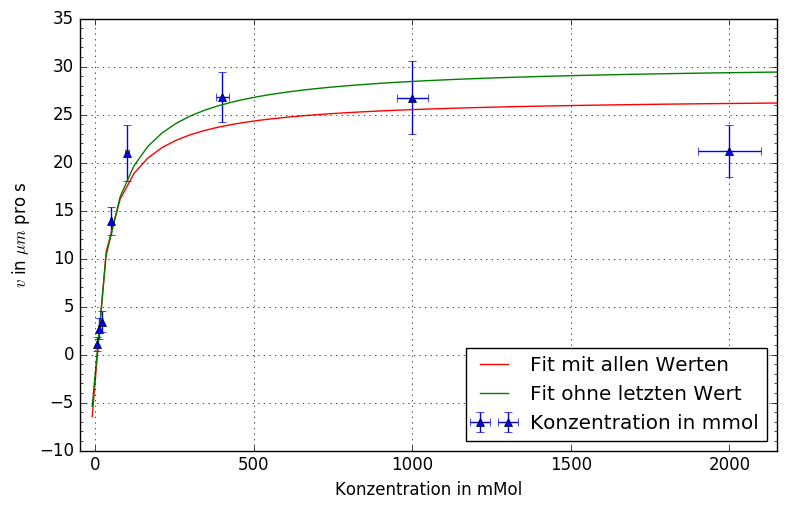
\includegraphics[width=0.8\textwidth]{bilder/both_fits.png}
  \caption{gemessene Aktingeschwindigkeit in $\sfrac{\mu m}{s}$ in A}
  \label{fig:normal_speed}
\end{figure}
Bereits bei der Versuchdurchführung war die geringe Geschwindigkeit der Filamente aufgefallen.
Diese Abweichung könnte auf einem nicht linearen Zusammenhang zwischen
Aktingeschwindikeit und Produktionsrate des ADP deuten.
Eine weiter Ursache für die niedrigen Geschwindigkeiten könnte ein Pippetierfehler sein,
der der dafür gesorgt hat, dass es eine andere ATP Konzentration in der Lösung gab.\newline 
Um die Nichtlinearität genauer zu untersuchen müsste man den Versuch erneut durchführen, 
mit mehr Abstufungen verschiedener Konzentrationen.
Bei der Wiederholung des Versuchs müsste man ebenso darauf achten genau zu pippetieren.
Wegen der ungenauen Datenlage kann man keinen einzelnen genauen Wert für die maximale
Aktingeschwindikgeit oder die Gleichgewichtskonstante angeben.
Es wurden zwei Fits durchgeführt, dabei wurde einmal der letzte Wert in den Fit mit einbezogen und einmal weggelassen. Da der äußerste Datenpunkt einer Messung oft nicht aussagekräftig ist,
werden die Werte vom Fit verwendet, der den äußersten Datenpunkt außenvorlässt.
Dennoch wurden beide Graphen gezeichnet, um die Integrität einer Wissenschaftlichen Arbeit zu bewahren.
Die Fit Werte des durchgehenden Graphen in Abbildung \ref{fig:normal_speed} sind $K_m = 66 \pm 17$ und $v_{max} = 30.3 \pm 2.3 \sfrac{\mu m}{s}$.\\ 
Verwendet man das Michaelis Menten Gesetz \ref{equ:michaelis_menten} und nimmt auf beiden seiten die Inverse gibt es den linearen Zusammenhang \ref{equ:michaelis_inverse}:
\begin{equation}
  \frac{1}{\nu} = \frac{K_m}{\nu_{max}} \cdot [S] + \frac{1}{\nu_{max}}
  \label{equ:michaelis_inverse}
\end{equation}
Somit lassen sich die Werte auch als Linearer Fit plotten, wie in Abbildug \ref{fig:1_over_speed}.
Der lineare Fit ergibt für $K_m = 158 \pm 109$ und $v_{max} = 39 \pm 29 \sfrac{\mu m}{s}$.
Man erkennt, dass die Unsicherheiten des Linearen fits
deutlich höher sind als die Unsicherheiten des Fits direkt nach der Formel.
Anhand der Fehlerbalken des Plots \ref{fig:1_over_speed} wird der Grund des schlechteren Fits ersichtlich. Der letzte Wert hat in der linearen keine starke Aussagekraft. Dennoch wird beim gewichtungslosen Fitten genauso viel Wert darauf gelegt, wie auf die anderen Werte.
Das bringt einen zu hohen Fehler in die Fitparameter hinein.
Für die künftige Arbeit als Wissenschaftler ist es von enormer Bedeutung die Fits mit den jeweiligen
Gewichtungen zu machen, um aussagekräftige Ergebnisse zu erzielen.
\begin{figure}[]
  \centering
  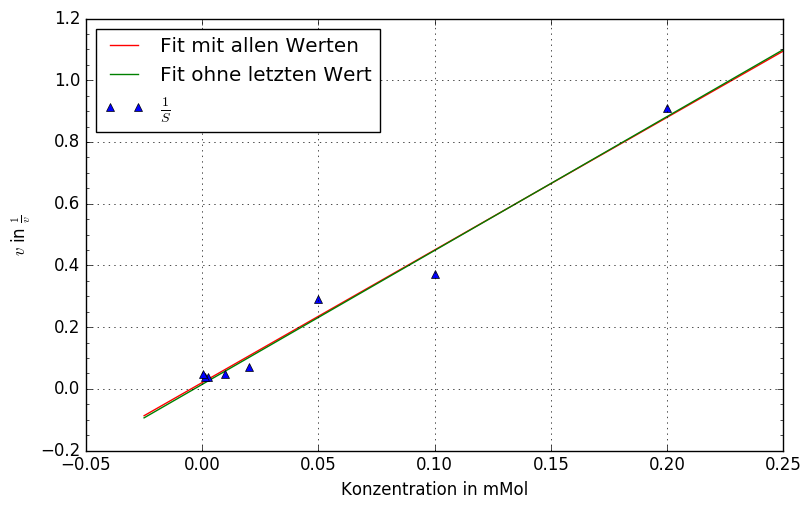
\includegraphics[width=0.8\textwidth]{bilder/both_fits_1over.png}
  \caption{Fit über 1/$\nu$  in $\sfrac{s}{\mu m}$ in A}
  \label{fig:1_over_speed}
\end{figure}

%%% Local Variables:
%%% mode: latex
%%% TeX-master: "../motors"
%%% End:
